% vim:ft=tex

\section{Data Profiling}

Data profiling is the process of reviewing source data, understanding structure, content and
interrelationships, and identifying potential for data projects. For the project, the Santander Bicycle data will be profiled more closely \citep{TFL2019}. For this I mainly used Zeppelin notebooks and the HDP cluster with four worker nodes initialized in chapter \ref{intallhadoop}. Zeppelin works similar to Jupyter notebooks and also supports magic commands. However, Zeppelin stores the notebooks in .json format, while Jupyter notebooks (python) uses \textbf{.ipynb}. A corresponding import of Zeppelin notebooks into Jupyter is therefore not possible and
should be considered when working with one of them. Furthermore, as already mentioned, HDP only
supports python 2.7.x, so all Python code in Zeppelin is python 2.7.x as well. (The Nominatim server and
Django already use Python 3.7.x).
\subsection{Data Preparation}
The Santander bicycle data is available on the public Transport for London TfL website.
The structure of these data is as followed:
\begin{itemize}
\item CycleCounters: has information about speed, bike details (length, wheels, axles, class...),
direction, timestamps and serial number.
\begin{itemize}
\item Blackfriars May and June and July
\item Embankment May and June and July
\end{itemize}
\item CycleParking: contains proprietary map material
\item CycleRoutes: contains geographical spatial data (GeoJSON) and .KML files
\item Usage-stats: information about rental stations, duration, start / end time
\end{itemize}
With regard to the folder structure shown above, CycleRoutes and Usage-stats are decisive. In
\glqq CycleCounters\grqq, apart from the maximum driven speed (56 mph!) with a borrowed Santander Cycle, no noteworthy information is contained. Therefore, only the CycleRoutes and Usage-stats data are
considered in the first step of Data Profiling. The CycleParking folder could contain useful map material,
but I only know from Google Earth that can read \textbf{.kml} files and that it is neither compatible with Geopandas nor with Nominatim. Most raw data are available either as .csv files or as .xlsx files.
One problem that arose when reading the usage-stats was that the folder contained 156 csv sheets and
each file was about 30 MB in size. Reading and concatenating as Pandas DataFrame unfortunately
completely occupied the maximum free memory of the master node, so the python job could not be
finished and was in an endless run mode. To work around the problem, we started a Spark job with the
PySpark API on the cluster instead of the Panda DataFrame. The spark job had created a DataFrame from
156 raw files within 12 seconds (i.e. it read 38.122.372 lines of raw text!). What we get here is a so called
Resilient Distributed Dataset (RDD) or Spark DataFrame which, in contrast to the Pandas DataFrame, is
redundant and distributed over the Cluster DataNodes. With the following PySpark method an RDD can
be generated:
\begin{figure}[H]
\hspace{-0.8cm}
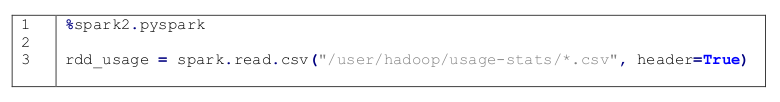
\includegraphics[width=1.1\textwidth]{img/spark1}\label{pic:spark1}
\end{figure}
\noindent Of course the files of the folder \glqq usage-stats\grqq need to be stored on HDFS before it can be read in with Spark. There are several ways of doing this, we used just a Zeppelin cell with magic command shell (\%sh) to execute shell based commands within the notebook. With that one can use:
\begin{lstlisting}[breaklines=true]
execute hdfs dfs -put
/home/hadoop/TFL_Cycling_Data_raw/usage-stats
/user/hadoop/usage-stats
\end{lstlisting}
to push the files on the datanodes of HDP. Remember the default replication size of Hadoop is 3, i.e. the
files are replicated on three worker nodes but not on fur, which should still be resilient enough.
The next decisive step is to prepare the usage-stats data and clean it up a bit. If we read in the data as
described above, our Spark DataFrame has the following columns:
\begin{lstlisting}[language=bash,breaklines=true]
|Rental Id|Duration|Bike Id| End Date|EndStation Id| EndStation Name|
Start Date|StartStation Id| StartStation Name|
\end{lstlisting}
Since we only want to plot the bicycle stations at this time, the Rental ID columns and the date columns
have been removed. This has the advantage that the DataFrame is already smaller and we don't carry any
unnecessary ballast. Furthermore, NaN values have been replaced by mandatory \glqq 0\grqq and duplicates have been removed. The TFL also offers numerous .xml based live feeds, from which we can get the coordinates (longitude and latitude) to the rental stations. We can also use this to fetch the coordinates:
\begin{figure}[H]
\hspace{-0.8cm}
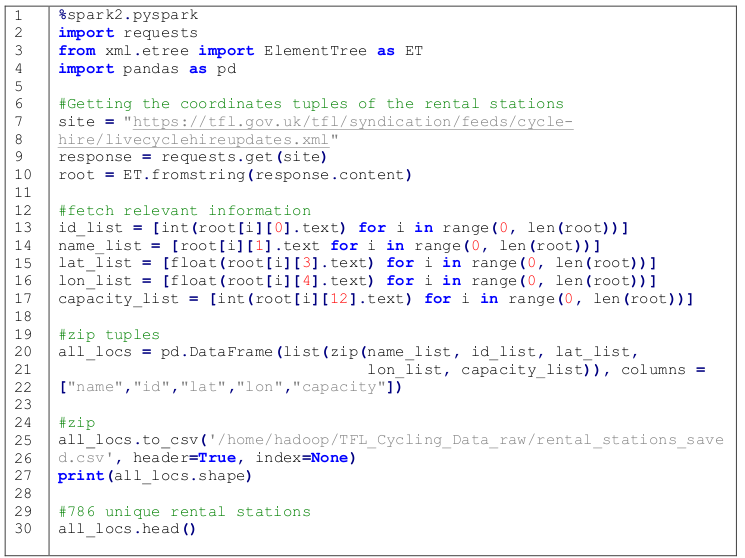
\includegraphics[width=1.1\textwidth]{img/spark2}\label{pic:spark2}
%\captionof{figure}{}
\end{figure}
\noindent This gives us not only the longitude and latitude, but also the maximum bicycle capacity of any station in London. This information could still be quite useful. As you can see, we have 786 unique bicycle stations in London (which are quite a lot).
Remark: Livecyclehireupdates.xml contains also following attributes:
\begin{itemize}
\item installed
\item locked
\item installDate
\item nbBikes
\item nbEmptyDocks
\item nbDocks
\end{itemize}
Given that there are 786 stations across London (at least at the time of writing), this allows for 786 * 785 = 617.010 possible journey combinations if we ignore those that start and end at the same station. The
next step is some data cleansing steps such as sorting, renaming and converting data types. PySpark offers
similar operations for the RDDs as for Pandas DataFrames. However, some pandas such as \glqq iloc()\grqq cannot
be transferred to Spark RDDs. Therefore Spark offers the option to directly execute SQL queries in
DataFrames. Anyway, the fetched data from the live feed must still be merged with the rdd\_usage Spark
DataFrame. For this purpose we first saved the Pandas DataFrame locally and then uploaded it to the
HDFS. This checkpoint is then read in again with PySpark as RDD. Merging works similar to SQL or/and
python. To do this, simply use the \glqq join\grqq command to link the two DataFrames:
\begin{figure}[H]
\hspace{-0.8cm}
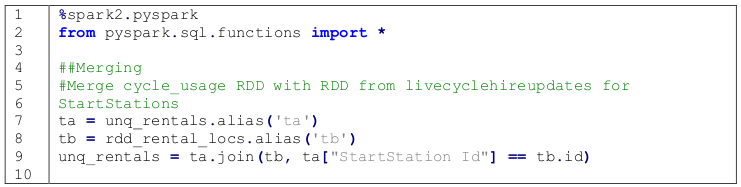
\includegraphics[width=1.1\textwidth]{img/spark3}\label{pic:spark3}
\end{figure}
\noindent In this case we also used alias (similar to the alias of SQL) in order to shorten the joining function name. The rest of the merging stuff is automatically done by the Spark API. After all the data
munging steps we got following schema of our combined and prepared usage-stats table:
\begin{lstlisting}[breaklines=true]
StartStation Id|EndStation latitude|StartStation Id|Duration|StartStation longitude|StartStation
Address|StartStation capacity| EndStation Address|EndStation latitude|EndStation longitude|EndStation capacity|
\end{lstlisting}
One can note, that there are also the columns \glqq StartStation ID Used\grqq and \glqq EndStation ID Used\grqq which stands for frequency of rented bikes on a single station. This gives us an indication of how
popular the station is in comparison with other ones. It might be also used as a weighting factor
for plotting on maps which will be described in just a moment.
With this, we can begin to plot statistics. But at first let compare the size of the new file with the
total size of all loaded cycle-usages. The total size was around 5.4 GB (which could not be simply
loaded into a Pandas DataFrame) whereas the new DataFrame has only 0.9 GB size. The reduction
of the size can be explained by the fact that we removed some unused columns and dropped
duplicates. This means also we are now able to use Pandas because to load 1 GB into a local
memory should be possible for most common computers. In fact, the Hadoop test environment
has shown its functionality and legitimation for the using in big data projects.
\begin{figure}[H]
\hspace{-0.8cm}
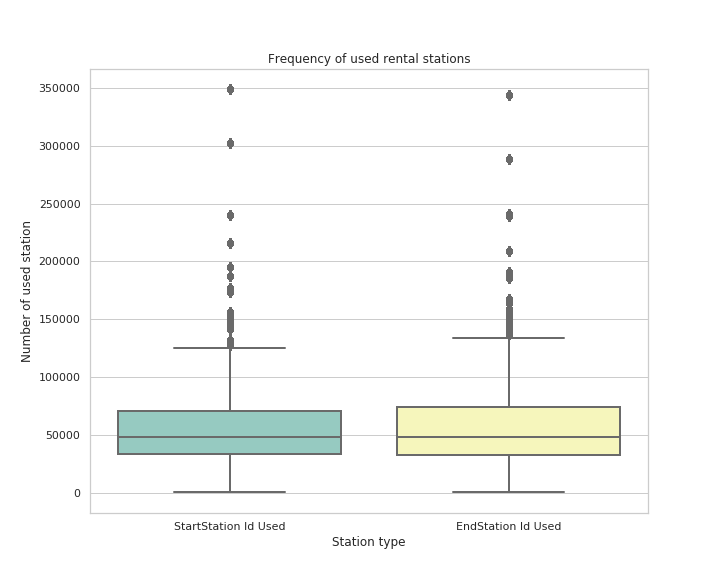
\includegraphics[width=1.1\textwidth]{img/plot1}
\captionof{figure}{Frequency of used StartStations and EndStations}\label{pic:plot1}
\end{figure}
\noindent As we can see from Figure \ref{pic:plot1}, the use of end stations slightly outweighs the starting stations,
which merely means that more different end stations than different start stations
were used. Apparently there are some very popular rental stations like the outliers from figure
\ref{pic:plot1} show. It is worth noting that the data were all collected from 2016 - 2018. (The year 2014-2016 are not included in this case). 
The next plot should serve us to show the density center of the rental stations locations. For this a joint
kernel density estimation plot could be helpful. We are plotting longitude against latitude of each single
StartStation. The illustrations looks then like this:
\begin{figure}[H]
\hspace{-0.8cm}
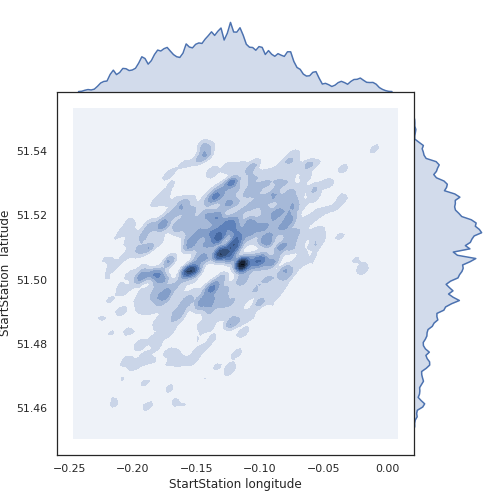
\includegraphics[width=1.1\textwidth]{img/plot2}\label{pic:plot2}
\captionof{figure}{Frequency of used StartStations and EndStations}\label{pic:plot2}
\end{figure}
\noindent 
The centroid or center of this plot is indicated by the dark spots. There are the most rental stations as also the frequency distributions (i.e. histograms) on the right border and on the top are clearly showing. Apart from that center of gravity, on the right corner there are also rental stations placed (guessing between longitude: -0,01 and latitude 51,6) which indicates that these rental stations must be placed in an outer borough of London. At a next, it would be useful to show the rental stations on a map based on their usage. As already mentioned we have 786 unique rental stations so that we can drop the duplicates for this case. In fact, we have saved the number of used stations on a separate column. At this step we prefer to use Jupyter on a local machine since Zeppelin on the cluster is not supporting IPython Display which is required by third-party packages such as folium. So we loaded the prepared cycle-usage data into a local Pandas dataframe. Now we can plot a heatmap for the rental stations:
\begin{figure}[H]
\hspace{-0.8cm}
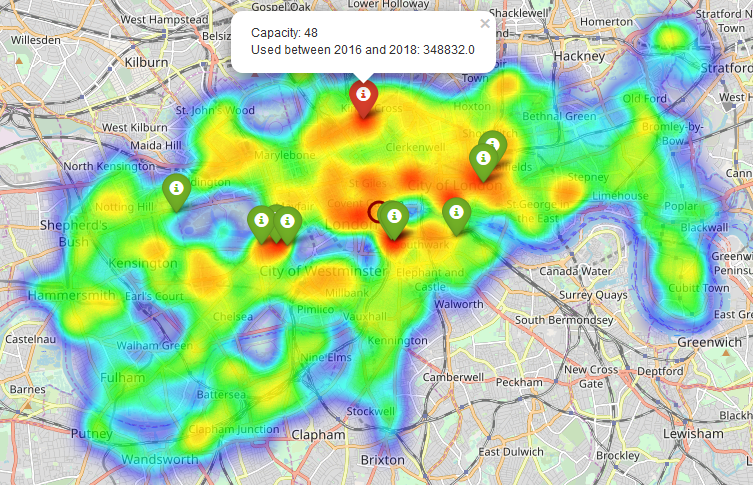
\includegraphics[width=1.1\textwidth]{img/heat}\label{pic:heat}
\captionof{figure}{Top 10 used Santander rental stations}\label{pic:heat}
\end{figure}
\noindent 
The red marker in figure \ref{pic:heat} indicates the most often used bicycle station in London in last two years. This is not surprisingly because close to the biking station there is London train station. Probably many travelers who are arriving by train are using a Santander cycle. However, this interactive map has been saved and uploaded on a webserver on the Hadoop cluster (\href{http://i-hadoop-01.informatik.hs-ulm.de/most_stations.html}{link})
As we can see, there are many rental stations close together. For a first impression this should be enough
as one can already see the capacity of each single Santander rental bike station by clicking on the marker
and also the location of each station is visible on the map. As an addition one can see the frequency of
each station by looking at the sizes of the heat spots or/and reading marker details.
\subsection{Conclusion of the file sizing problem}
\begin{enumerate}
\item The sizing problem can be well handled by Spark
\item The HDP is working and storing the cycle-usage files on HDFS
\item For plotting tasks packages like folium or seaborn cannot be used with Spark DataFrame
\begin{itemize}
\item Converting back to Pandas DF might exceed local RAM
\item Using Jupyter notebook on local computer for plotting maps (e.g. folium)
\end{itemize}
\end{enumerate}
\subsection{CyclingRoutes}
The Cycling routes from the folder of TFL [24] are geojson files and represent real geographical
routes within London inner city.
There are 5 \emph{geojson} files in this folder available:
\begin{itemize}
\item \emph{Central\_London\_Grid.json}
\begin{itemize}
\item \emph{Central London Grid}: i s a set of safer, connected routes for cyclists across central London
\end{itemize}
\item \emph{Mini\_Hollands.json}
\begin{itemize}
\item Mini-Hollands have features that make cycling feel safer and more convenient.
\end{itemize}
\item \emph{Quietways.json}
\begin{itemize}
\item \emph{Quietways} are signposted cycle routes, run on quieter back streets to provide for those cyclists who want to travel at a more relaxed pace.
\end{itemize}
\item \emph{super-highways-quietways.json}
\begin{itemize}
\item \emph{Combination of super highways and quietways}
\end{itemize}
\item \emph{Cycle\_Superhighways.json}
\begin{itemize}
\item \emph{Cycle\_Superhighways} are on main roads and often segregate cyclists from other
traffic.
\end{itemize}
\end{itemize}
The routes should be concatenated by a single GeoPandas GeoDataFrame. Doing so requires to read the
geojson files with following scripts:
\subsection{Plotting Data}
Let’s see if we can compare the frequency of used rental stations between StartStation and EndStation.
We can not use swarm plots or any other kind of plots with fine granular details since \glqq matplotlib\grqq or Python would try to draw over six million dots which will easily exceed the local RAM of the master node. Beside from that, we also would see to many points at the same location since lot of stations are drawn several times. A better plot in my opinion is to use a box plot as following figure shows:
\begin{figure}[H]
\hspace{-0.8cm}
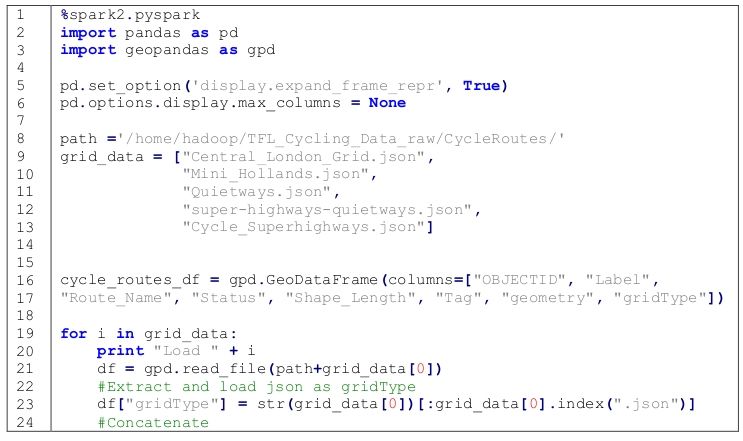
\includegraphics[width=1.1\textwidth]{img/spark4}\label{pic:spark4}
\end{figure}
\begin{figure}[H]
\hspace{-0.8cm}
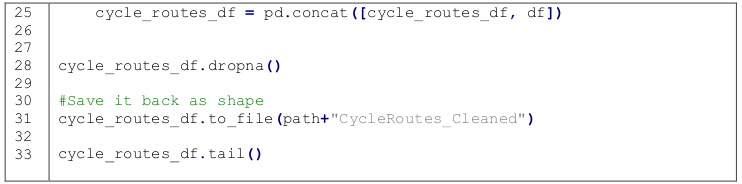
\includegraphics[width=1.1\textwidth]{img/spark5}\label{pic:spark5}
\end{figure}
\noindent So we get in only GeoPandas DataFrame which contains the 5 Cycling routes. In addition, the type of each route was stored in the column \glqq gridType\grqq, so that it can be filtered later for certain routes. For a first plot a Choropleth should show the different routes.
\subsection{Conclusion}
\begin{enumerate}
\item The data lacks in documentation and quality (Data Preperation \& Cleansing necessary).
\item Some column names can be misunderstood (e.g. SITE\_NUMBER <> SITE\_ID).
\item Data like SPEED or SPEED\_MHP should be stored in one way.
\item Many columns like the axles are not meaningful and useful for our project. (e.g. Cyclecounters
has 107 columns!)
\item Raw data seems not to be complete (e.g. only May, June, July)
\item \emph{usage-stats} is very big. Necessity to use all usage-stats?
\end{enumerate}
In the next sprint we will create similar plots as shown above, but this time with duplicates and times in mind. Because it is quite often the case that between two same bicycle stations several same entries exist at different times with different rental periods. For example, a use case would be to display the day/night change on the map,
i.e. do more cyclists ride quietways or super-highways at night between rental stations?
